\chapter{Case Studies}
\label{ch:case-studies}

\missing

\section{Multi-iteration Path Profiling}
\label{se:kblpp-case-studies}
In this section we consider examples of applications where $k$-iteration path profiling can reveal optimization opportunities or help developers comprehend relevant properties of a piece of software by identifying structured execution patterns that would be missed by an acyclic-path profiler. Our discussion is based on idealized examples found in real programs of the kind of behavior that can be exploited using multi-iteration path profiles. Since our methodology can be applied to different languages, we addressed both Java and C applications\footnote{We profiled Java programs using the k-BLPP tool described in \missing\ and C programs with manual source code instrumentation based on a C implementation of the algorithms and data structures of Section\missing, available at \url{http://www.dis.uniroma1.it/~demetres/kstream/}. }.

\subsection{Masked Convolution Filters in Image Processing}
\label{ss:convolution}

\begin{figure}[!ht]
\centering
\cprotect\fbox{
\begin{minipage}{10cm}
\begin{small}
\begin{verbatim}
 #define NEIGHBOR(m,i,dy,dx,w)                 \
     (*((m)+(i)+(dy)*(w)+(dx)))

 #define CONVOLUTION(i) do {                   \
     val  = NEIGHBOR(img_in, (i),              \
                     -2, -2, cols)*filter[0];  \
     val += NEIGHBOR(img_in, (i),              \
                     -2, -1, cols)*filter[1];  \
     ...
     val += NEIGHBOR(img_in, (i),
                     +2, +2, cols)*filter[24]; \
     val = val*factor+bias;                    \
     img_out[i] = (unsigned char)              \
        (val < 0 ? 0 : val > 255 ? 255 : val); \
 } while(0)

 void filter_conv(unsigned char* img_in,
                  unsigned char* img_out,
                  unsigned char* mask,
                  char filter[25],
                  double factor, double bias,
                  int rows, int cols) {
     int val;
     long n = rows*cols, i;

     for (i = 0; i < n; i++)
         if (mask[i]) img_out[i] = img_in[i];
         else CONVOLUTION(i);
 }
\end{verbatim}
\end{small}
\end{minipage}
}
\vspace{-2mm}
\caption{Masked image filtering code based on a convolution matrix.}
\label{fig:CS-convolution-orig}
\end{figure}

As a first example, we consider a classic application of convolution filters to image processing, addressing the problem of masked filtering that arises when the user applies a transformation to a collection of arbitrary-shaped subregions of the input image. A common scenario is face anonymization, illustrated in the example of \myfigure\ref{fig:CS-convolution-images}. The case study discussed in this section shows that $k$-iteration path profiling with large values of $k$ can identify regular patterns spanning multiple loop iterations that can be effectively exploited to speed up the code. 

\myfigure\ref{fig:CS-convolution-orig} shows a C implementation of a masked image filtering algorithm based on a $5\times 5$ convolution matrix\footnote{The source code of our example is provided at \url{http://www.dis.uniroma1.it/~demetres/kstream/}.}. The function takes as input a grayscale input image (8-bit depth) and a black and white mask image that specifies the regions of the image to be filtered. \myfigure\ref{fig:CS-convolution-images} shows a sample input image (top), a mask image (center), and the output image (bottom) generated by the code of \myfigure\ref{fig:CS-convolution-orig} by applying a blur filter to the regions of the input image specified by the mask. Notice that the filter code iterates over all pixels of the input image and for each pixel checks if the corresponding mask is black (zero) or white (non-zero, i.e., 255). If the mask is white, the original grayscale value is copied from the input image to the output image; otherwise, the grayscale value of the output pixel is computed by applying the convolution kernel to the neighborhood of the current pixel in the input image. To avoid expensive boundary checks in the convolution operation, the mask is preliminarily cropped so that all values near the border are white (this operation takes negligible time).

\myfigure\ref{fig:CS-convolution-kipf} shows a portion of the $10$-IPF forest containing the trees rooted at the BL path IDs that correspond to: the path entering the loop (ID=0), the copy branch taken in the loop body when the mask is non-zero (ID=1), and the convolution branch taken in the loop body when the mask is zero (ID=2). The $10$-IPF was generated on the workload of \myfigure\ref{fig:CS-convolution-images} and was pruned by removing all nodes whose counters are less than $0.01\%$ of the counter of their parents or less than $0.01\%$ of the counter of their roots. For each node $v$ in the forest, if $v$ has a counter that is $X\%$ of the counter of its parent and is $Y\%$ of the counter of the root, then the edge leading to $v$ is labeled with ``$X\% (Y\%)$''. A visual analysis of the forest shows that:
\begin{itemize}[itemsep=0pt,parsep=3pt]
\item the copy branch (1) is more frequent than the convolution branch (2);
\item 98.9\% of the times a copy branch (1) is taken, it is repeated consecutively at least 10 times, and only $0.1\%$ of the times is immediately followed by a convolution branch;
\item 95\% of the times a convolution branch (2) is taken, it is repeated consecutively at least 10 times, and only $0.6\%$ of the times is immediately followed by a copy branch.
\end{itemize}

\ifdefined\noauthorea
\begin{figure}[!t]
\centerline{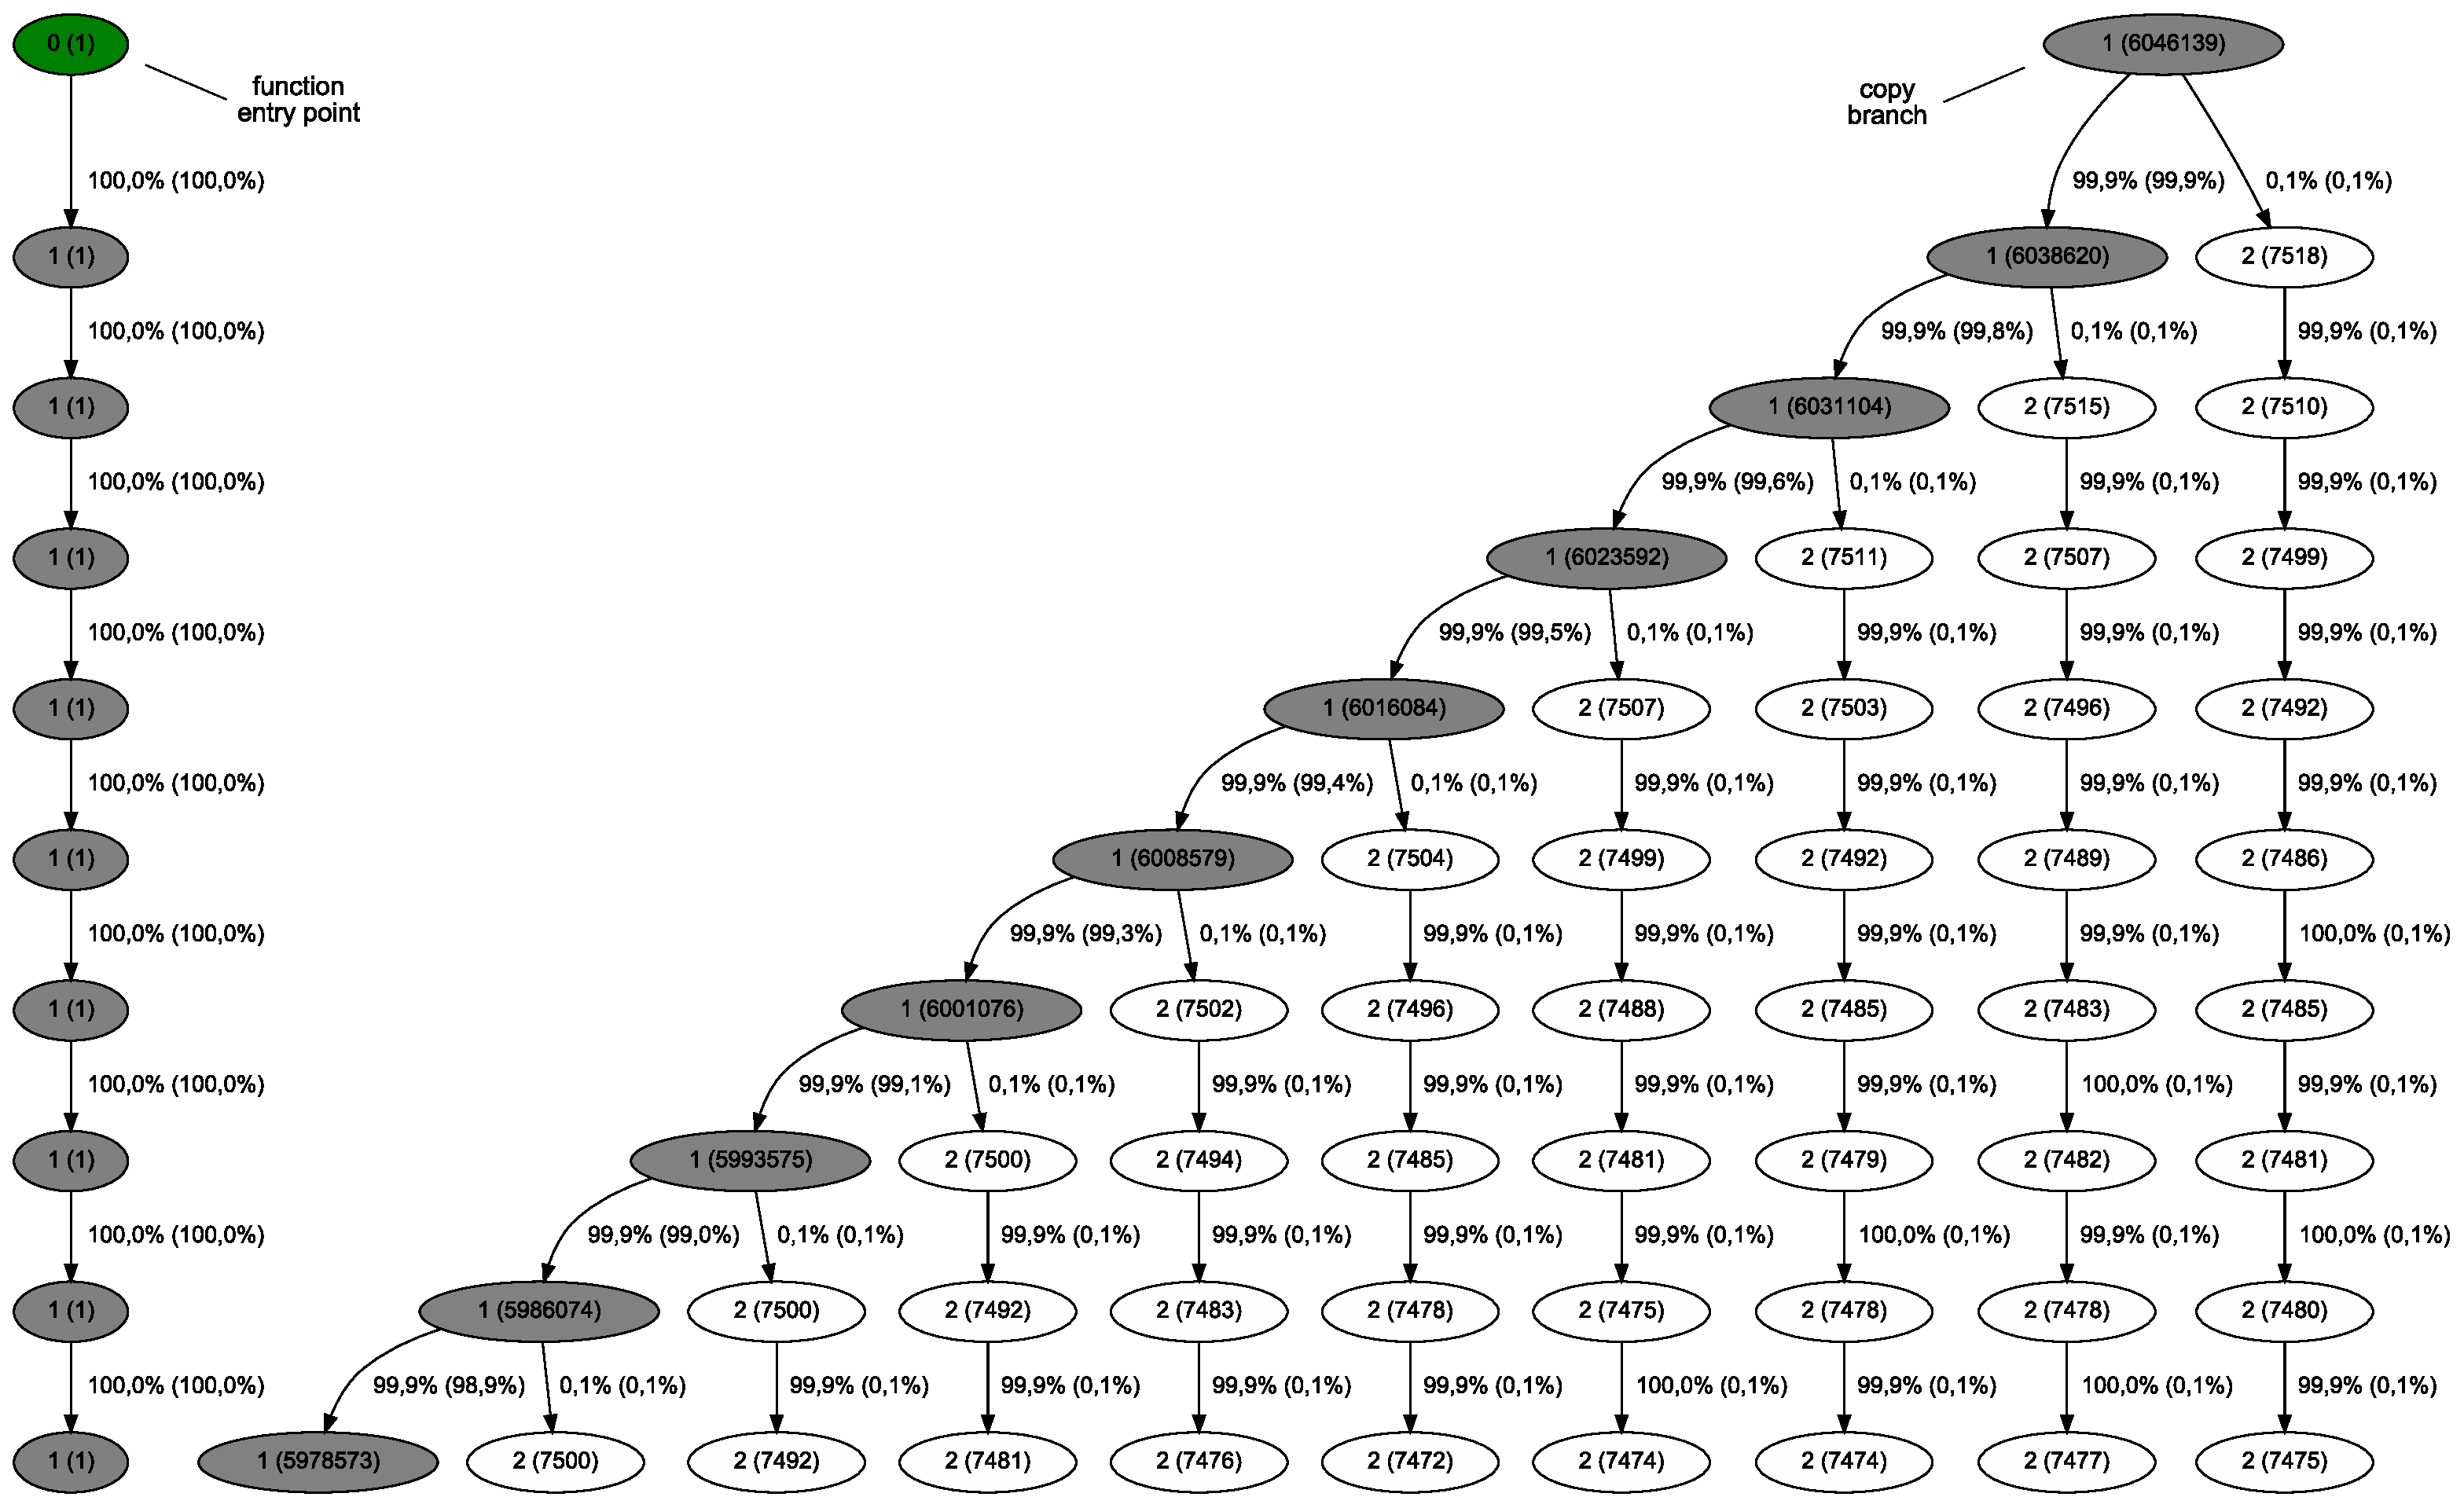
\includegraphics[width=0.95\textwidth]{figures/CS-kipf-indiana/CS-kipf-indiana-top.eps}}
\vspace{6mm}
\centerline{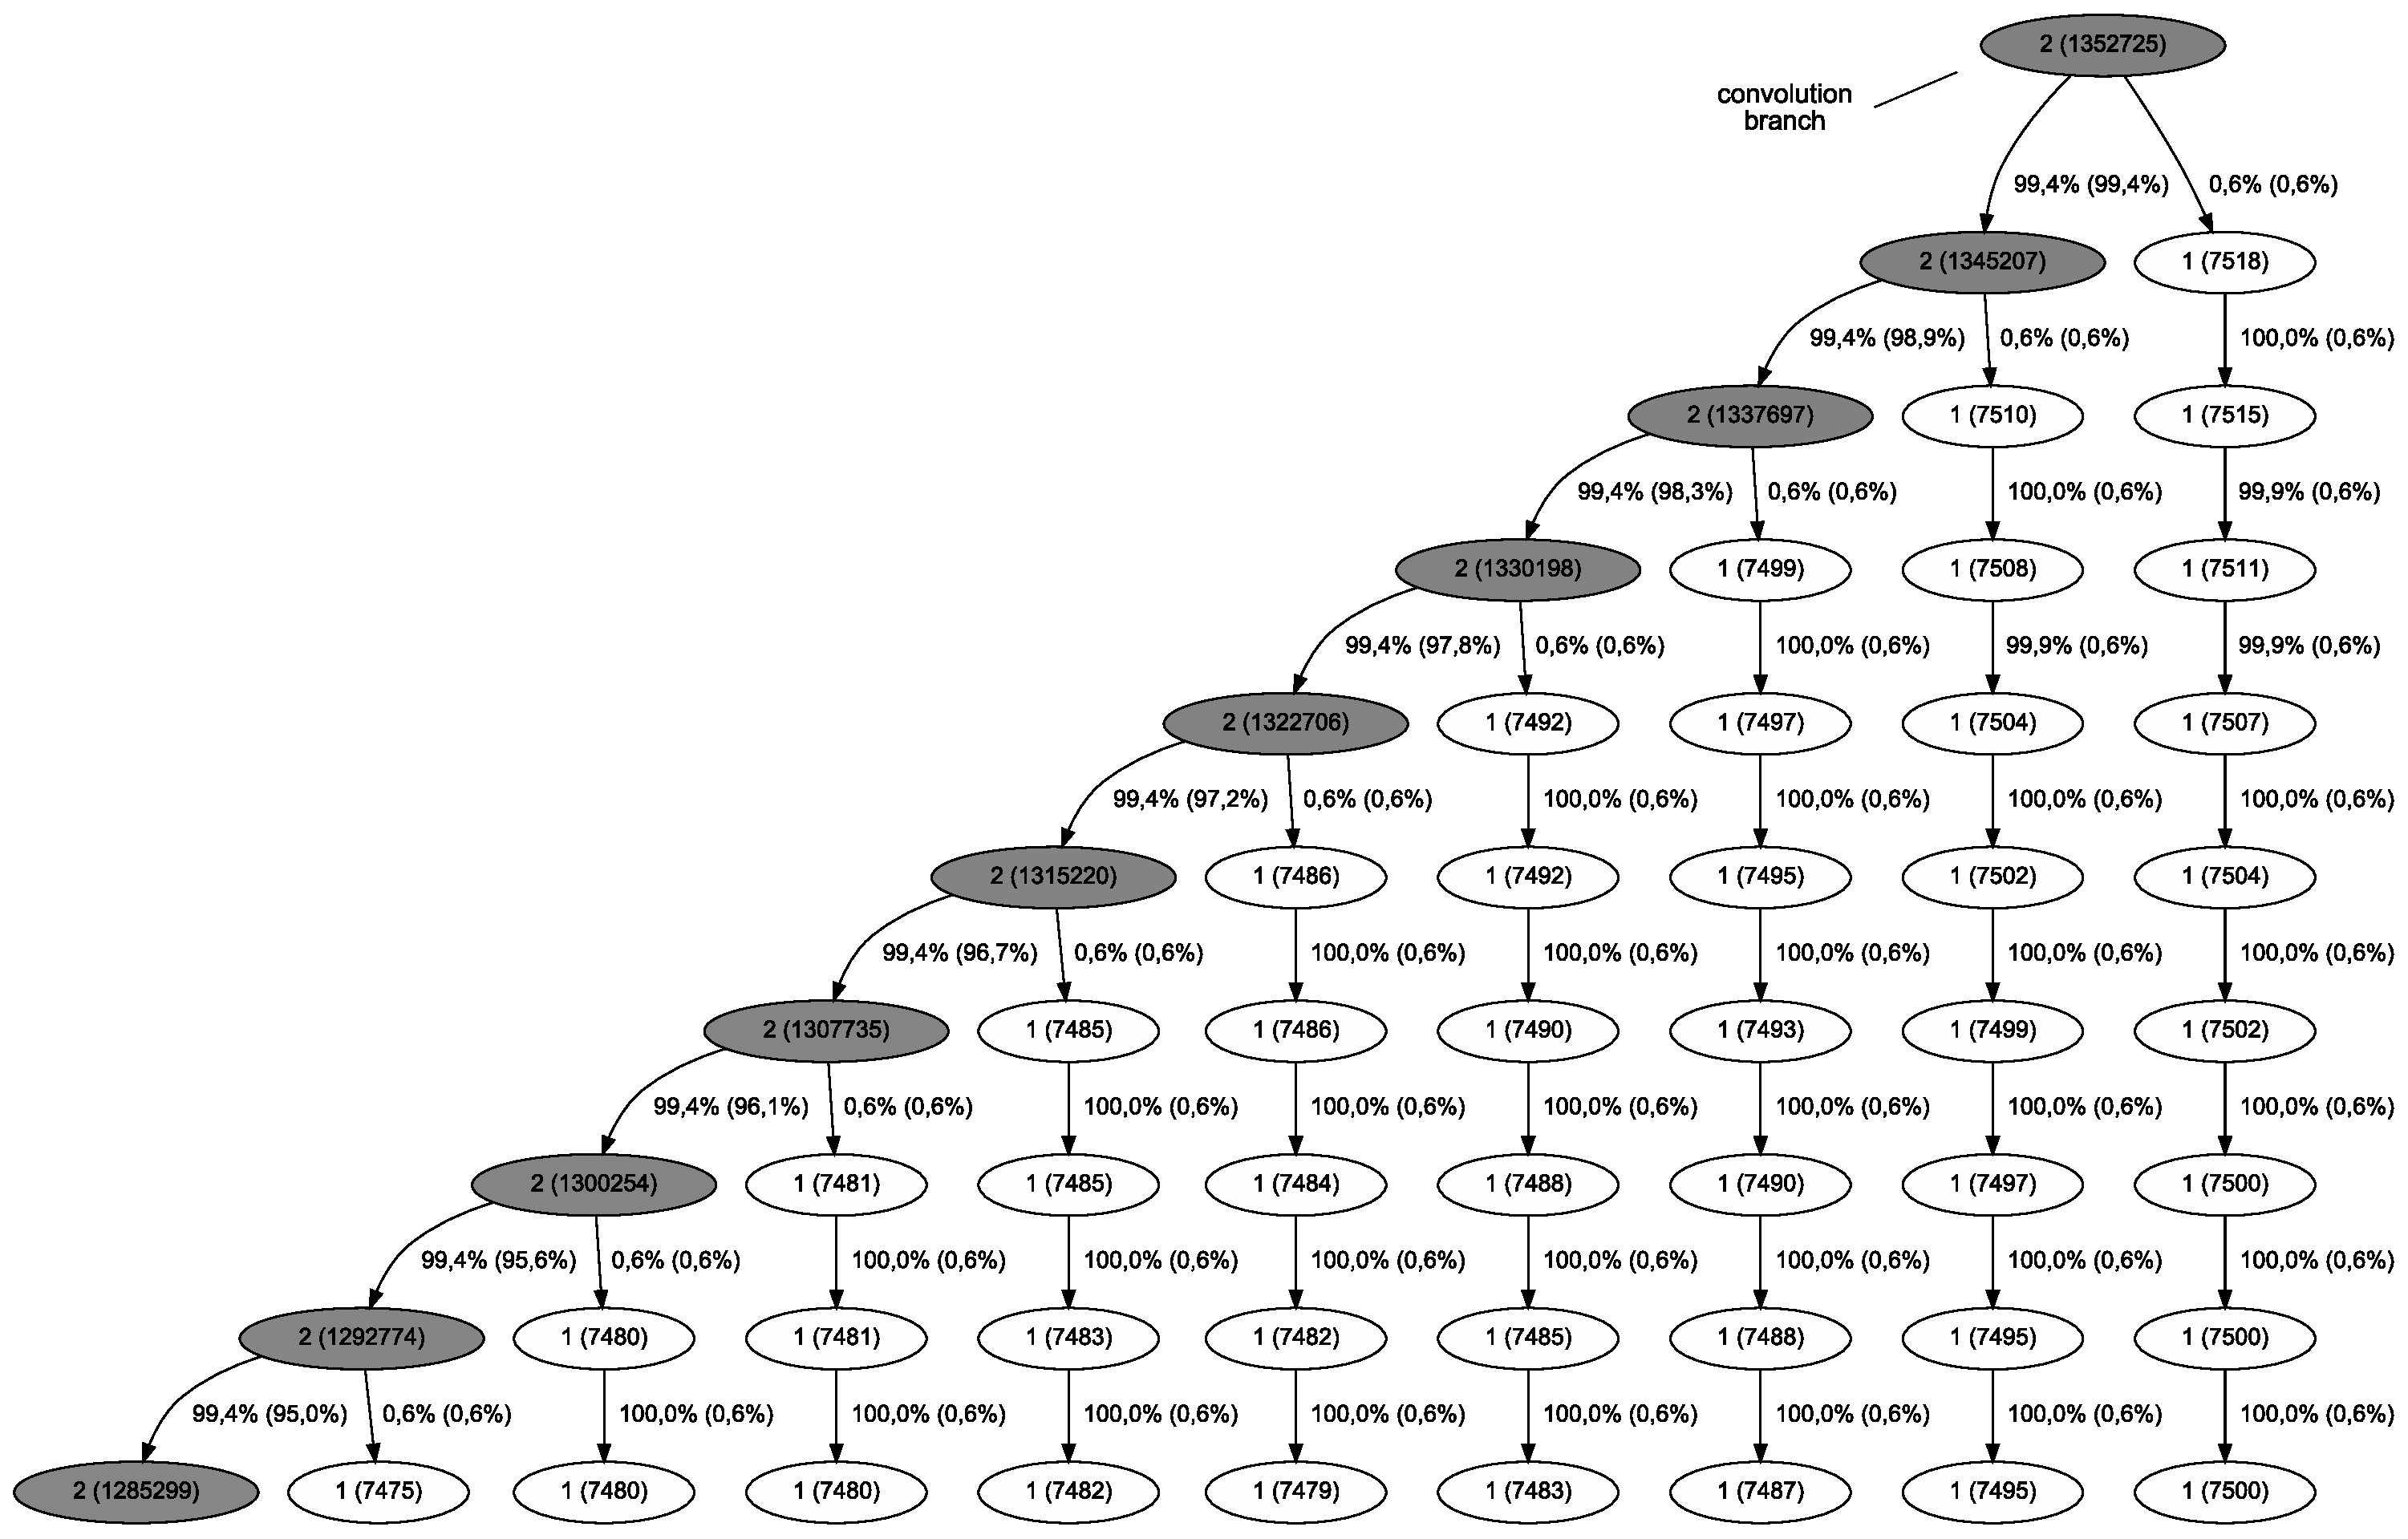
\includegraphics[width=0.95\textwidth]{figures/CS-kipf-indiana/CS-kipf-indiana-bottom.eps}}
\caption{\protect\label{fig:CS-convolution-kipf} $10$-IPF forest of the code of \myfigure\ref{fig:CS-convolution-orig} on the workload of \myfigure\ref{fig:CS-convolution-images}.

}
\end{figure}
\fi

\ifdefined\noauthorea
\begin{figure}[!t]
\begingroup\setlength{\fboxsep}{0pt}
\centerline{\framebox{\includegraphics[width=0.6\textwidth]{figures/CS-indiana-pacers/CS-indiana-pacers-orig.png}}}
\vspace{2.5mm}
\centerline{\framebox{\includegraphics[width=0.6\textwidth]{figures/CS-indiana-pacers/CS-indiana-pacers-mask.png}}}
\vspace{2.5mm}
\centerline{\framebox{\includegraphics[width=0.6\textwidth]{figures/CS-indiana-pacers/CS-indiana-pacers-out.png}}}
\endgroup
\caption{\protect\label{fig:CS-convolution-images} Masked blur filter example: original $3114\times2376$ image (top), filter mask (center), filtered image (bottom).


}
\end{figure}
\fi

\noindent This entails that both the copy and the convolution operations are repeated along long consecutive runs. The above properties are typical of masks used in face anonymization and other common image manipulations based on user-defined selections of portions of the image. The collected profiles suggest that consecutive iterations of the same branches may be selectively unrolled as shown in \myfigure\ref{fig:CS-convolution-opt}. Each iteration of the outer loop, designed for a 64-bit platform, works on 8 (rather than 1) pixels at a time. Three cases are possible:

\begin{enumerate}[itemsep=0pt,parsep=3pt]
\item the next 8 mask entries are all 255 (white): the 8 corresponding input pixel values are copied to the output image at once with a single assignment instruction;
\item the next 8 mask entries are all 0 (black): the kernel is applied sequentially to each of the next 8 input pixels;
\item the next 8 mask entries are mixed: an inner loop performs either copy or convolution on the corresponding pixels.
\end{enumerate}

\begin{figure}[!ht]
\centering
\cprotect\fbox{
\begin{minipage}{10cm}
\begin{small}
\begin{verbatim}
 for (i = 0; i < n-7; i += 8) {

    if (*(long*)(mask+i) == 0xFFFFFFFFFFFFFFFF)
       *(long*)(img_out+i) = *(long*)(img_in+i);

    else if (*(long*)(mask+i) == 0) {
       CONVOLUTION(i);
       CONVOLUTION(i+1);
       CONVOLUTION(i+2);
       CONVOLUTION(i+3);
       CONVOLUTION(i+4);
       CONVOLUTION(i+5);
       CONVOLUTION(i+6);
       CONVOLUTION(i+7);
    }

    else for (j = i; j < i+8; j++)
       if (mask[j]) img_out[j] = img_in[j];
       else CONVOLUTION(j);
 }
\end{verbatim}
\end{small}
\end{minipage}
}
\vspace{-2mm}
\caption{Optimized 64-bit version of the loop of \myfigure\ref{fig:CS-convolution-orig}.}
\label{fig:CS-convolution-opt}
\end{figure}

\subsubsection*{Performance analysis}
To assess the benefits of the optimization performed in \myfigure\ref{fig:CS-convolution-opt}, we conducted several tests on recent commodity platforms (Intel Core 2 Duo, Intel Core i7, Linux and MacOS X, 32 and 64 bits, {\tt gcc} -O3), considering a variety of sample images and masks with regions of different sizes and shapes. We obtained non-negligible speedups on all our tests, with a peak of about 21\% on the workload of \myfigure\ref{fig:CS-convolution-images} ($3114\times2376$ pixels) and about 30\% on a larger $9265\times7549$ image with a memory footprint of about 200 MB. In general, the higher the white entries in the mask, the faster the code, with larger speedups on more recent machines. As we expected, for entirely black masks the speedup was instead barely noticeable: this is due to the fact that the convolution operations are computationally demanding and tend to hide the benefits of loop unrolling.

\subsubsection*{Discussion}
The example discussed in this section shows that both the ability to profile paths across multiple iterations, and the possibility to handle large values of $k$ played a crucial role in optimizing the code. Indeed, acyclic-path profiling would count the number of times each branch is taken, but would not reveal that they appear in consecutive runs. Moreover, previous multi-iteration approaches that only handle very small values of $k$ would not capture the long runs that make the proposed optimization effective. 

For the example of \myfigure\ref{fig:CS-convolution-images}, an acyclic-path profile would indicate that the copy branch is taken 81.7\% of the times, but not how branches are interleaved. From this information, we would be able to deduce that the average length of a sequence of consecutive white values in the mask is $\ge$ 4. Our profile shows that, 98.9\% of the times the actual length is at least 10, fully justifying our optimization that copies 8 bytes at a time. The advantage of $k$-iteration path profiling increases for masks with a more balanced ratio between white and black pixels: for a 50-50 ratio, an acyclic-path profile would indicate that the average length of consecutive white/black runs is $\ge$ 1, yielding no useful information for loop unrolling purposes.

The execution pattern where the same branches are repeatedly taken over consecutive loop iterations is common to several other applications, which may benefit from optimizations that take advantage of long repeated runs. For instance, the {\tt LBM\_performStreamCollide} function of the {\tt lbm} benchmark from the \speccpu\ suite iterates over a 3D domain, simulating incompressible fluid dynamics based on the Lattice Boltzmann Method. An input geometry file specifies obstacles that determine a steady state solution. The loop contains branches that depend upon the currently scanned cell, which alternates between obstacles and void regions of the domain, producing a \kipf\ similar to that of \myfigure\ref{fig:CS-convolution-kipf} on typical workloads.

\section{Optimizing Higher-Order Functions in MATLAB}